\documentclass{article}

% content/resources/templates/preamble.tex
\usepackage[margin=0.6in]{geometry}
\author{Milav Dabgar}
\usepackage{amsmath,amssymb,amsthm}
\usepackage{booktabs}
\usepackage{multirow}
\usepackage{xcolor}
\usepackage{tcolorbox}
\tcbuselibrary{breakable,skins}
\usepackage[colorlinks=true,linkcolor=blue]{hyperref}
\usepackage{titlesec}
\usepackage{enumitem}
\usepackage{tikz}
\usepackage{pgfplots}
\usepackage{circuitikz}
\usepackage[version=4]{mhchem}
\usepackage{longtable}
\usepackage{array}
\usepackage{float}
\usepackage{caption}
\usepackage{listings}

\lstset{
  basicstyle=\small\ttfamily,
  breaklines=true,
  breakatwhitespace=false,
  postbreak=\mbox{\textcolor{red}{$\hookrightarrow$}\space},
  float=false,
  numbers=left,
  numberstyle=\tiny\color{gray},
  numbersep=10pt,
  xleftmargin=2em,
  keywordstyle=\color{blue},
  commentstyle=\color{green!60!black},
  stringstyle=\color{purple},
  backgroundcolor=\color{gray!5},
  showstringspaces=false,
  tabsize=2,
  captionpos=b,
  keepspaces=true,
  columns=flexible
}

\pgfplotsset{compat=1.18}
\usetikzlibrary{shapes,arrows,positioning,calc,patterns,decorations.pathmorphing,decorations.markings,arrows.meta}

% Color scheme
\definecolor{headcolor}{RGB}{0,102,204}
\definecolor{keycolor}{RGB}{220,20,60}
\definecolor{solutioncolor}{RGB}{34,139,34}
\definecolor{mnemoniccolor}{RGB}{148,0,211}
\definecolor{codecolor}{RGB}{0,0,100}

% Spacing
\setlength{\parskip}{3pt}
\setlist[itemize]{nosep}
\setlist[enumerate]{nosep}

% Title formatting
\titleformat{\section}{\Large\bfseries\color{headcolor}}{\thesection}{1em}{}
\titleformat{\subsection}{\large\bfseries\color{headcolor}}{\thesubsection}{1em}{}

% Pandoc tightlist compatibility
\providecommand{\tightlist}{%
  \setlength{\itemsep}{0pt}\setlength{\parskip}{0pt}}

% Pandoc longtable compatibility
\newcounter{none}
\def\thenone{}


% content/resources/templates/english-boxes.tex

% Custom environments
\newtcolorbox{solutionbox}{
 breakable,
 enhanced,
 colback=solutioncolor!5!white,
 colframe=solutioncolor!75!black,
 fonttitle=\bfseries,
 title=Solution
}

\newtcolorbox{solutionboxnobreak}{
 colback=solutioncolor!5!white,
 colframe=solutioncolor!75!black,
 fonttitle=\bfseries,
 title=Solution
}

\newtcolorbox{keyformula}{
 breakable,
 enhanced,
 colback=keycolor!5!white,
 colframe=keycolor!75!black,
 fonttitle=\bfseries,
 title=Key Formula
}

\newtcolorbox{mnemonicboxenv}{
 breakable,
 enhanced,
 colback=mnemoniccolor!5!white,
 colframe=mnemoniccolor!75!black,
 fonttitle=\bfseries,
 title=Mnemonic
}

\newcommand{\mnemonicbox}[1]{%
  \begin{mnemonicboxenv}
    #1
  \end{mnemonicboxenv}
}


% Custom commands for GTU solutions
% This file defines semantic commands for consistent formatting

% Question command with automatic formatting
\newcommand{\question}[2]{%
  \section*{Question #1}%
  \textbf{#2}%
}

% OR question variant
\newcommand{\questionor}[2]{%
  \section*{Question #1 OR}%
  \textbf{#2}%
}

% Proper table environment with caption
\newenvironment{answertable}[1]{%
  \begin{table}[htbp]
  \centering
  \caption{#1}
}{%
  \end{table}
}

% Proper figure environment for diagrams
\newenvironment{answerdiagram}[1]{%
  \begin{figure}[htbp]
  \centering
  \caption{#1}
}{%
  \end{figure}
}

% Semantic markup for key terms
\newcommand{\keyword}[1]{\textbf{#1}}
\newcommand{\code}[1]{\texttt{#1}}
\newcommand{\classname}[1]{\texttt{#1}}
\newcommand{\methodname}[1]{\texttt{#1}}

% Proper quotation marks
\newcommand{\mnemonic}[1]{``#1''}

\usetikzlibrary{shapes.multipart, chains, arrows.meta, positioning, calc}

\title{Data Structure And Application (1333203) - Summer 2024 Solution}
\date{June 12, 2024}

\begin{document}
\maketitle

\questionmarks{1(a)}{3}{Define linear data structure and give its examples.}

\begin{solutionbox}
A linear data structure is a collection of elements arranged in sequential order where each element has exactly one predecessor and one successor (except first and last elements).

\begin{center}
\captionof{table}{Linear Data Structures Examples}
\begin{tabulary}{\linewidth}{|L|L|}
\hline
\textbf{Data Structure} & \textbf{Description} \\ \hline
\textbf{Array} & Fixed-size collection of elements accessed by index \\ \hline
\textbf{Linked List} & Chain of nodes with data and reference to next node \\ \hline
\textbf{Stack} & LIFO (Last In First Out) structure \\ \hline
\textbf{Queue} & FIFO (First In First Out) structure \\ \hline
\end{tabulary}
\end{center}
\end{solutionbox}

\begin{mnemonicbox}
\mnemonic{ALSQ are in a Line}
\end{mnemonicbox}

\questionmarks{1(b)}{4}{Define time and space complexity.}

\begin{solutionbox}
Time and space complexity measure algorithm efficiency in terms of execution time and memory usage as input size grows.

\begin{center}
\captionof{table}{Complexity Comparison}
\begin{tabulary}{\linewidth}{|L|L|L|L|}
\hline
\textbf{Complexity Type} & \textbf{Definition} & \textbf{Measurement} & \textbf{Importance} \\ \hline
\textbf{Time Complexity} & Measures execution time required by an algorithm as a function of input size & Big O notation (O(n), O(1), O(n^2)) & Determines how fast an algorithm runs \\ \hline
\textbf{Space Complexity} & Measures memory space required by an algorithm as a function of input size & Big O notation (O(n), O(1), O(n^2)) & Determines how much memory an algorithm needs \\ \hline
\end{tabulary}
\end{center}
\end{solutionbox}

\begin{mnemonicbox}
\mnemonic{TS: Time-Speed and Space-Storage}
\end{mnemonicbox}

\questionmarks{1(c)}{7}{Explain the concept of class and object with example.}

\begin{solutionbox}
Classes and objects are fundamental OOP concepts where classes are blueprints for creation objects with attributes and behaviors.

\begin{center}
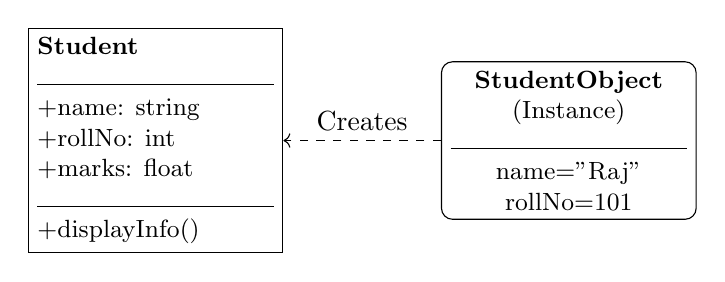
\begin{tikzpicture}[class/.style={rectangle, draw, minimum width=3cm, align=left, font=\small}]
    % Class Student using standard node with tabular for better formatting
    \node [class] (student) {
        \textbf{Student} \\
        \rule{3cm}{0.5pt} \\
        +name: string \\
        +rollNo: int \\
        +marks: float \\
        \rule{3cm}{0.5pt} \\
        +displayInfo()
    };
    
    % Object StudentObject
    \node [class, rounded corners, right=2cm of student, align=center] (obj) {
        \textbf{StudentObject} \\
        (Instance) \\
        \rule{3cm}{0.5pt} \\
        name="Raj" \\
        rollNo=101
    };
    
    \draw [->, dashed] (obj) -- node[above] {Creates} (student);
\end{tikzpicture}
\captionof{figure}{Class and Object Relationship}
\end{center}

\begin{lstlisting}[language=Python, caption={Class and Object Example}]
class Student:
    def __init__(self, name, rollNo, marks):
        self.name = name
        self.rollNo = rollNo
        self.marks = marks
    
    def displayInfo(self):
        print(f"Name: {self.name}, Roll No: {self.rollNo}, Marks: {self.marks}")

# Creating object
student1 = Student("Raj", 101, 85.5)
student1.displayInfo()
\end{lstlisting}

\begin{itemize}
    \item \textbf{Class}: Blueprint defining attributes (name, rollNo, marks) and methods (displayInfo)
    \item \textbf{Object}: Instance (student1) created from the class with specific values
\end{itemize}
\end{solutionbox}

\begin{mnemonicbox}
\mnemonic{CAR - Class defines Attributes and Routines}
\end{mnemonicbox}

\questionmarks{1(c) OR}{7}{Explain instance method, class method and static method with example.}

\begin{solutionbox}
Python supports three method types: instance, class, and static methods, each serving different purposes.

\begin{center}
\captionof{table}{Comparison of Method Types}
\begin{tabulary}{\linewidth}{|L|L|L|L|L|}
\hline
\textbf{Method Type} & \textbf{Decorator} & \textbf{First Parameter} & \textbf{Purpose} & \textbf{Access} \\ \hline
\textbf{Instance Method} & None & self & Operate on instance data & Can access/modify instance state \\ \hline
\textbf{Class Method} & @classmethod & cls & Operate on class data & Can access/modify class state \\ \hline
\textbf{Static Method} & @staticmethod & None & Utility functions & Cannot access instance or class state \\ \hline
\end{tabulary}
\end{center}

\begin{lstlisting}[language=Python, caption={Method Types Example}]
class Student:
    school = "ABC School"  # class variable
    
    def __init__(self, name):
        self.name = name  # instance variable
    
    def instance_method(self):  # instance method
        return f"Hi {self.name} from {self.school}"
    
    @classmethod
    def class_method(cls):  # class method
        return f"School is {cls.school}"
    
    @staticmethod
    def static_method():  # static method
        return "This is a utility function"
\end{lstlisting}
\end{solutionbox}

\begin{mnemonicbox}
\mnemonic{ICS: Instance-Self, Class-Cls, Static-Solo}
\end{mnemonicbox}

\questionmarks{2(a)}{3}{Explain concept of recursive function.}

\begin{solutionbox}
A recursive function is a function that calls itself during its execution to solve smaller instances of the same problem.

\begin{center}
\begin{tikzpicture}[level distance=1.5cm, sibling distance=2cm]
    \node [gtu state] (A) {factorial(3)};
    \node [gtu state, below=of A] (B) {factorial(2)};
    \node [gtu state, below=of B] (C) {factorial(1)};
    \node [below=of C] (D) {Return 1};
    
    \draw [->] (A) -- (B);
    \draw [->] (B) -- (C);
    \draw [->] (C) -- (D);
    \draw [->, bend right=45] (D.east) to node[right] {Return 1*1=1} (C.east);
    \draw [->, bend right=45] (C.east) to node[right] {Return 2*1=2} (B.east);
    \draw [->, bend right=45] (B.east) to node[right] {Return 3*2=6} (A.east);
\end{tikzpicture}
\captionof{figure}{Recursive Function Execution}
\end{center}
\end{solutionbox}

\begin{mnemonicbox}
\mnemonic{BASE and RECURSE - Base case stops, Recursion repeats}
\end{mnemonicbox}

\questionmarks{2(b)}{4}{Define stack and queue.}

\begin{solutionbox}
Stack and queue are linear data structures with different access patterns for data insertion and removal.

\begin{center}
\captionof{table}{Stack vs Queue}
\begin{tabulary}{\linewidth}{|L|L|L|}
\hline
\textbf{Feature} & \textbf{Stack} & \textbf{Queue} \\ \hline
\textbf{Access Pattern} & LIFO (Last In First Out) & FIFO (First In First Out) \\ \hline
\textbf{Operations} & Push (insert), Pop (remove) & Enqueue (insert), Dequeue (remove) \\ \hline
\textbf{Access Points} & Single end (top) & Two ends (front, rear) \\ \hline
\textbf{Visualization} & Like plates stacked vertically & Like people in a line \\ \hline
\textbf{Applications} & Function calls, undo operations & Print jobs, process scheduling \\ \hline
\end{tabulary}
\end{center}
\end{solutionbox}

\begin{mnemonicbox}
\mnemonic{SLIFF vs QFIFF - Stack-LIFO vs Queue-FIFO}
\end{mnemonicbox}

\questionmarks{2(c)}{7}{Explain basic operations on stack.}

\begin{solutionbox}
Stack operations follow LIFO (Last In First Out) principle.

\begin{center}
\captionof{table}{Stack Operations}
\begin{tabulary}{\linewidth}{|L|L|L|}
\hline
\textbf{Operation} & \textbf{Description} & \textbf{Time Complexity} \\ \hline
\textbf{Push} & Insert element at the top & O(1) \\ \hline
\textbf{Pop} & Remove element from the top & O(1) \\ \hline
\textbf{Peek/Top} & View top element without removing & O(1) \\ \hline
\textbf{isEmpty} & Check if stack is empty & O(1) \\ \hline
\textbf{isFull} & Check if stack is full & O(1) \\ \hline
\end{tabulary}
\end{center}

\begin{center}
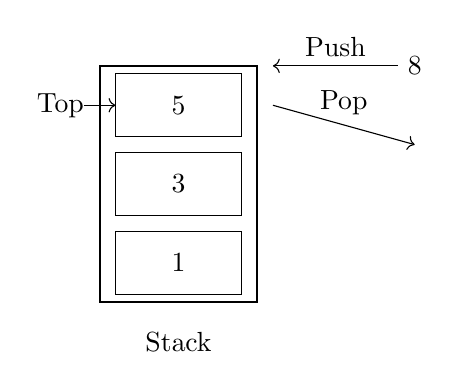
\begin{tikzpicture}
    % Stack drawing
    \draw [thick] (0,0) -- (0,3) -- (2,3) -- (2,0) -- cycle;
    \foreach \y/\val in {0.5/1, 1.5/3, 2.5/5}
        \draw (0.2, \y-0.4) rectangle (1.8, \y+0.4) node[midway] {\val};
    
    \node at (1, -0.5) {Stack};
    \node at (-0.5, 2.5) {Top};
    \draw [->] (-0.2, 2.5) -- (0.2, 2.5);
    
    % Push
    \node (push) at (4, 3) {8};
    \draw [->] (push) -- node[above] {Push} (2.2, 3);
    
    % Pop
    \draw [->] (2.2, 2.5) -- node[above] {Pop} (4, 2);
\end{tikzpicture}
\captionof{figure}{Stack Push and Pop}
\end{center}

\begin{lstlisting}[language=Python, caption={Stack Implementation}]
class Stack:
    def __init__(self):
        self.items = []
    
    def push(self, item):
        self.items.append(item)
    
    def pop(self):
        if not self.isEmpty():
            return self.items.pop()
    
    def peek(self):
        if not self.isEmpty():
            return self.items[-1]
    
    def isEmpty(self):
        return len(self.items) == 0
\end{lstlisting}
\end{solutionbox}

\begin{mnemonicbox}
\mnemonic{PIPES - Push In, Pop Exit, See top}
\end{mnemonicbox}

\questionmarks{2(a) OR}{3}{Define singly linked list.}

\begin{solutionbox}
A singly linked list is a linear data structure with a collection of nodes where each node contains data and a reference to the next node.

\begin{center}
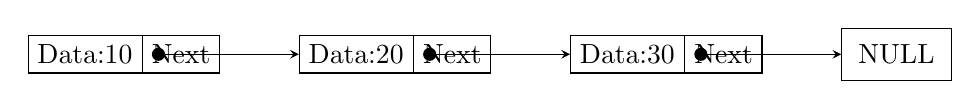
\begin{tikzpicture}[list/.style={rectangle split, rectangle split parts=2, draw, rectangle split horizontal}, >=stealth, start chain]
  \node[list, on chain] (A) {Data:10 \nodepart{second} Next};
  \node[list, on chain] (B) {Data:20 \nodepart{second} Next};
  \node[list, on chain] (C) {Data:30 \nodepart{second} Next};
  \node[on chain, draw, inner sep=6pt] (D) {NULL};
  \draw[*->] let \p1 = (A.two), \p2 = (A.center) in (\x1,\y2) -- (B);
  \draw[*->] let \p1 = (B.two), \p2 = (B.center) in (\x1,\y2) -- (C);
  \draw[*->] let \p1 = (C.two), \p2 = (C.center) in (\x1,\y2) -- (D);
\end{tikzpicture}
\captionof{figure}{Singly Linked List}
\end{center}
\end{solutionbox}

\begin{mnemonicbox}
\mnemonic{DNL - Data and Next Link}
\end{mnemonicbox}

\questionmarks{2(b) OR}{4}{Explain Enqueue and Dequeue operations on Queue.}

\begin{solutionbox}
Enqueue and Dequeue are the primary operations for adding and removing elements in a queue data structure.

\begin{center}
\captionof{table}{Queue Operations}
\begin{tabulary}{\linewidth}{|L|L|L|L|}
\hline
\textbf{Operation} & \textbf{Description} & \textbf{Implementation} & \textbf{Time Complexity} \\ \hline
\textbf{Enqueue} & Add element at the rear end & queue.append(element) & O(1) \\ \hline
\textbf{Dequeue} & Remove element from the front end & element = queue.pop(0) & O(1) linked list, O(n) array \\ \hline
\end{tabulary}
\end{center}

\begin{center}
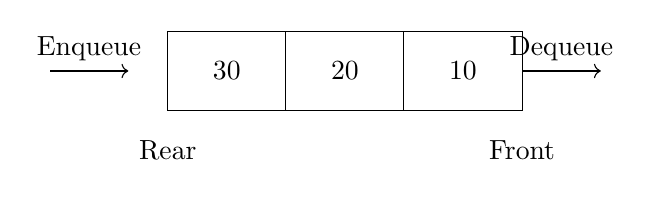
\begin{tikzpicture}
    % Queue
    \foreach \x/\val in {0/30, 1.5/20, 3/10}
        \draw (\x, 0) rectangle (\x+1.5, 1) node[midway] {\val};
    
    \node at (0, -0.5) {Rear};
    \node at (4.5, -0.5) {Front};
    
    % Enqueue
    \draw [<-] (-0.5, 0.5) -- node[above] {Enqueue} (-1.5, 0.5);
    
    % Dequeue
    \draw [->] (4.5, 0.5) -- node[above] {Dequeue} (5.5, 0.5);
\end{tikzpicture}
\captionof{figure}{Queue Operations}
\end{center}
\end{solutionbox}

\begin{mnemonicbox}
\mnemonic{ERfDFr - Enqueue at Rear, Dequeue from Front}
\end{mnemonicbox}

\questionmarks{2(c) OR}{7}{Convert expression A+B/C+D to postfix and evaluate postfix expression using stack assuming some values for A, B, C and D.}

\begin{solutionbox}
Converting and evaluating the expression "A+B/C+D" using stack:

\textbf{Step 1: Convert to Postfix}

\begin{center}
\captionof{table}{Infix to Postfix Conversion}
\begin{tabulary}{\linewidth}{|C|L|L|L|}
\hline
\textbf{Symbol} & \textbf{Stack} & \textbf{Output} & \textbf{Action} \\ \hline
A & & A & Add to output \\ \hline
+ & + & A & Push to stack \\ \hline
B & + & A B & Add to output \\ \hline
/ & + / & A B & Push to stack (higher prec) \\ \hline
C & + / & A B C & Add to output \\ \hline
+ & + & A B C / & Pop /, push + \\ \hline
D & + & A B C / + D & Add to output \\ \hline
End & & A B C / + D + & Pop remaining \\ \hline
\end{tabulary}
\end{center}
\textbf{Final Postfix:} $A B C / + D +$

\textbf{Step 2: Evaluate with values A=5, B=10, C=2, D=3}

\begin{center}
\captionof{table}{Postfix Evaluation}
\begin{tabulary}{\linewidth}{|C|L|L|}
\hline
\textbf{Symbol} & \textbf{Stack} & \textbf{Calculation} \\ \hline
5 (A) & 5 & Push value \\ \hline
10 (B) & 5, 10 & Push value \\ \hline
2 (C) & 5, 10, 2 & Push value \\ \hline
/ & 5, 5 & $10/2 = 5$ \\ \hline
+ & 10 & $5+5 = 10$ \\ \hline
3 (D) & 10, 3 & Push value \\ \hline
+ & 13 & $10+3 = 13$ \\ \hline
\end{tabulary}
\end{center}
\textbf{Result:} 13
\end{solutionbox}

\begin{mnemonicbox}
\mnemonic{PC-SE - Push operands, Calculate when operators, Stack holds Everything}
\end{mnemonicbox}

\questionmarks{3(a)}{3}{Enlist applications of Linked List.}

\begin{solutionbox}
\begin{center}
\captionof{table}{Applications of Linked List}
\begin{tabulary}{\linewidth}{|L|L|}
\hline
\textbf{Application} & \textbf{Why Linked List is Used} \\ \hline
\textbf{Dynamic Memory Allocation} & Efficient insertion/deletion without reallocation \\ \hline
\textbf{Implementing Stacks \& Queues} & Can grow and shrink as needed \\ \hline
\textbf{Undo Functionality} & Easy to add/remove operations from history \\ \hline
\textbf{Hash Tables} & For handling collisions via chaining \\ \hline
\textbf{Music Playlists} & Easy navigation between songs (next/previous) \\ \hline
\end{tabulary}
\end{center}
\end{solutionbox}

\begin{mnemonicbox}
\mnemonic{DSUHM - Dynamic allocation, Stacks \& queues, Undo, Hash tables, Music players}
\end{mnemonicbox}

\questionmarks{3(b)}{4}{Explain creation of singly linked list in python.}

\begin{solutionbox}
Creating a singly linked list in Python involves defining a Node class and implementing basic operations.

\begin{lstlisting}[language=Python, caption={Creating Linked List}]
class Node:
    def __init__(self, data):
        self.data = data
        self.next = None

class LinkedList:
    def __init__(self):
        self.head = None
    
    def append(self, data):
        new_node = Node(data)
        # If empty list, set new node as head
        if self.head is None:
            self.head = new_node
            return
        # Traverse to the end and add node
        last = self.head
        while last.next:
            last = last.next
        last.next = new_node
\end{lstlisting}

\begin{center}
\begin{tikzpicture}
    \node [gtu state] (node) {Create Node};
    \node [gtu state, right=of node] (head) {Set Head};
    \node [gtu state, right=of head] (traverse) {Traverse};
    \node [gtu state, right=of traverse] (attach) {Attach};
    
    \draw [gtu arrow] (node) -- (head);
    \draw [gtu arrow] (head) -- (traverse);
    \draw [gtu arrow] (traverse) -- (attach);
\end{tikzpicture}
\captionof{figure}{Creation Process}
\end{center}
\end{solutionbox}

\begin{mnemonicbox}
\mnemonic{CHEN - Create nodes, Head first, End attachment, Next pointers}
\end{mnemonicbox}

\questionmarks{3(c)}{7}{Write a code to insert a new node at the beginning and end of singly linked list.}

\begin{solutionbox}
\begin{lstlisting}[language=Python, caption={Insertion Operations}]
class Node:
    def __init__(self, data):
        self.data = data
        self.next = None

class LinkedList:
    def __init__(self):
        self.head = None
    
    # Insert at beginning (prepend)
    def insert_at_beginning(self, data):
        new_node = Node(data)
        new_node.next = self.head
        self.head = new_node
    
    # Insert at end (append)
    def insert_at_end(self, data):
        new_node = Node(data)
        if self.head is None:
            self.head = new_node
            return
        current = self.head
        while current.next:
            current = current.next
        current.next = new_node
\end{lstlisting}

\begin{center}
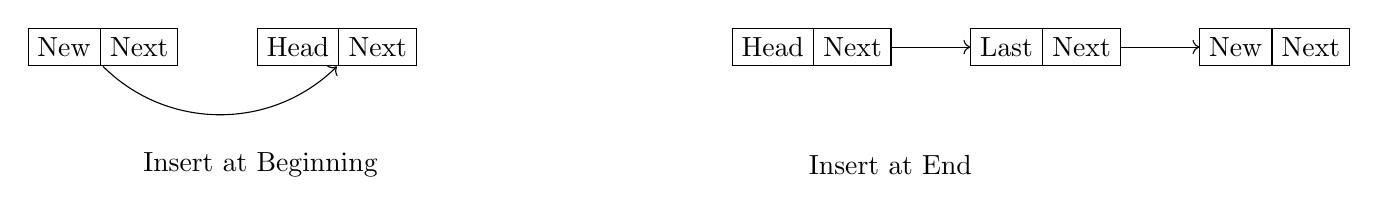
\begin{tikzpicture}[list/.style={rectangle split, rectangle split parts=2, draw, rectangle split horizontal}]
    % Insert at Beginning
    \node (new1) [list] {New \nodepart{second} Next};
    \node (head1) [list, right=1cm of new1] {Head \nodepart{second} Next};
    \draw [->] (new1.south) to[out=-45, in=-135] (head1.south);
    \node at (2, -1.5) {Insert at Beginning};

    % Insert at End
    \node (head2) [list, right=4cm of head1] {Head \nodepart{second} Next};
    \node (last) [list, right=1cm of head2] {Last \nodepart{second} Next};
    \node (new2) [list, right=1cm of last] {New \nodepart{second} Next};
    \draw [->] (head2) -- (last);
    \draw [->] (last) -- (new2);
    \node at (10, -1.5) {Insert at End};
\end{tikzpicture}
\captionof{figure}{Insertion Visualization}
\end{center}
\end{solutionbox}

\begin{mnemonicbox}
\mnemonic{BEN - Beginning is Easy and Next-based, End Needs traversal}
\end{mnemonicbox}

\questionmarks{3(a) OR}{3}{Write a code to count the number of nodes in singly linked list.}

\begin{solutionbox}
\begin{lstlisting}[language=Python, caption={Count Nodes}]
def count_nodes(self):
    count = 0
    current = self.head
    
    # Traverse the list and count nodes
    while current:
        count += 1
        current = current.next
    
    return count
\end{lstlisting}
\end{solutionbox}

\begin{mnemonicbox}
\mnemonic{CIT - Count Incrementally while Traversing}
\end{mnemonicbox}

\questionmarks{3(b) OR}{4}{Match appropriate options from column A and B}

\begin{solutionbox}
\begin{center}
\captionof{table}{Match Columns}
\begin{tabulary}{\linewidth}{|L|L|L|}
\hline
\textbf{Column A} & \textbf{Column B} & \textbf{Match} \\ \hline
1. Singly Linked List & c. Nodes contain data and reference to next & 1-c \\ \hline
2. Doubly Linked List & d. Nodes contain data, next and prev & 2-d \\ \hline
3. Circular Linked List & b. Last node points to first node & 3-b \\ \hline
4. Node & a. Basic unit containing data and references & 4-a \\ \hline
\end{tabulary}
\end{center}

\begin{center}
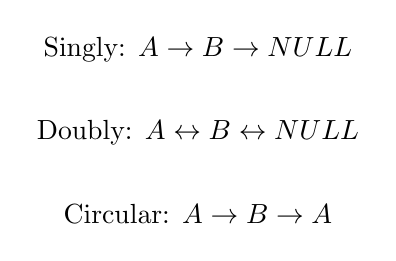
\begin{tikzpicture}[node distance=1.5cm]
    % Singly
    \node (S) {Singly: $A \rightarrow B \rightarrow NULL$};
    % Doubly
    \node [below=0.5cm of S] (D) {Doubly: $A \leftrightarrow B \leftrightarrow NULL$};
    % Circular
    \node [below=0.5cm of D] (C) {Circular: $A \rightarrow B \rightarrow A$};
\end{tikzpicture}
\captionof{figure}{Linked List Types}
\end{center}
\end{solutionbox}

\begin{mnemonicbox}
\mnemonic{SDCN - Single-Direction, Double-Direction, Circular-Connection, Node-Component}
\end{mnemonicbox}

\questionmarks{3(c) OR}{7}{Explain deletion of first and last node in singly linked list.}

\begin{solutionbox}
Deletion complexity depends on position.

\begin{center}
\captionof{table}{Deletion Comparison}
\begin{tabulary}{\linewidth}{|L|L|L|}
\hline
\textbf{Position} & \textbf{Approach} & \textbf{Complexity} \\ \hline
First Node & Change head pointer & O(1) \\ \hline
Last Node & Traverse to second-last node & O(n) \\ \hline
\end{tabulary}
\end{center}

\begin{lstlisting}[language=Python, caption={Deletion Code}]
def delete_first(self):
    if self.head is None: return
    self.head = self.head.next

def delete_last(self):
    if self.head is None: return
    if self.head.next is None:
        self.head = None
        return
    current = self.head
    while current.next.next:
        current = current.next
    current.next = None
\end{lstlisting}
\end{solutionbox}

\begin{mnemonicbox}
\mnemonic{FELO - First is Easy, Last needs One-before-last}
\end{mnemonicbox}

\questionmarks{4(a)}{3}{Explain concept of doubly linked list.}

\begin{solutionbox}
A doubly linked list is a bidirectional linear data structure.

\begin{center}
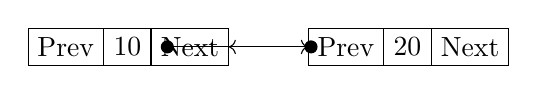
\begin{tikzpicture}[list/.style={rectangle split, rectangle split parts=3, draw, rectangle split horizontal}]
    \node[list] (A) {Prev \nodepart{second} 10 \nodepart{third} Next};
    \node[list, right=1cm of A] (B) {Prev \nodepart{second} 20 \nodepart{third} Next};
    \draw[*->] let \p1 = (A.three), \p2 = (A.center) in (\x1,\y2) -- (B);
    \draw[*->] let \p1 = (B.one), \p2 = (B.center) in (\x1,\y2) -- (A);
\end{tikzpicture}
\captionof{figure}{Doubly Linked List}
\end{center}
\end{solutionbox}

\begin{mnemonicbox}
\mnemonic{PDN - Previous, Data, Next}
\end{mnemonicbox}

\questionmarks{4(b)}{4}{Explain concept of linear search.}

\begin{solutionbox}
Linear search sequentially checks each element.

\begin{center}
\captionof{table}{Linear Search}
\begin{tabulary}{\linewidth}{|L|L|}
\hline
\textbf{Aspect} & \textbf{Description} \\ \hline
\textbf{Working} & Check each element start to end \\ \hline
\textbf{Time Complexity} & O(n) worst/average \\ \hline
\textbf{Best Case} & O(1) \\ \hline
\end{tabulary}
\end{center}

\begin{center}
\begin{tikzpicture}[node distance=2cm]
    \node [gtu state] (start) {Start};
    \node [gtu state, right=of start] (check) {Check Element};
    \node [gtu decision, right=of check] (match) {Match?};
    \node [gtu state, below=of match] (found) {Found};
    \node [gtu state, above=of match] (next) {Next};
    
    \draw [gtu arrow] (start) -- (check);
    \draw [gtu arrow] (check) -- (match);
    \draw [gtu arrow] (match) -- node[right] {Yes} (found);
    \draw [gtu arrow] (match) -- node[right] {No} (next);
    \draw [gtu arrow] (next) -| (check);
\end{tikzpicture}
\captionof{figure}{Linear Search Flow}
\end{center}
\end{solutionbox}

\begin{mnemonicbox}
\mnemonic{SCENT - Search Consecutively Each element until Target}
\end{mnemonicbox}

\questionmarks{4(c)}{7}{Write a code to implement binary search algorithm.}

\begin{solutionbox}
Binary search divides the search interval in half.

\begin{lstlisting}[language=Python, caption={Binary Search}]
def binary_search(arr, target):
    left = 0
    right = len(arr) - 1
    
    while left <= right:
        mid = (left + right) // 2
        
        if arr[mid] == target:
            return mid
        elif arr[mid] < target:
            left = mid + 1
        else:
            right = mid - 1
            
    return -1
\end{lstlisting}

\begin{center}
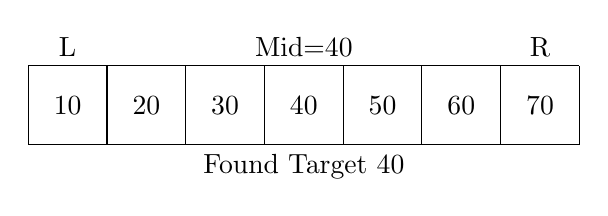
\begin{tikzpicture}
    \draw (0,0) grid (7,1);
    \foreach \x/\v in {0/10, 1/20, 2/30, 3/40, 4/50, 5/60, 6/70} \node at (\x+0.5, 0.5) {\v};
    \node [above] at (0.5, 1) {L};
    \node [above] at (6.5, 1) {R};
    \node [above] at (3.5, 1) {Mid=40};
    \node [below] at (3.5, 0) {Found Target 40};
\end{tikzpicture}
\captionof{figure}{Binary Search Execution}
\end{center}
\end{solutionbox}

\begin{mnemonicbox}
\mnemonic{MCLR - Middle Compare, Left or Right adjust}
\end{mnemonicbox}

\questionmarks{4(a) OR}{3}{Explain concept of selection sort algorithm.}

\begin{solutionbox}
Selection sort finds the minimum element and places it at the beginning.

\begin{itemize}
    \item \textbf{Time Complexity}: $O(n^2)$
    \item \textbf{Space Complexity}: $O(1)$
    \item \textbf{Method}: Find smallest, swap with current position.
\end{itemize}
\end{solutionbox}

\begin{mnemonicbox}
\mnemonic{FSMR - Find Smallest, Move to Right position, Repeat}
\end{mnemonicbox}

\questionmarks{4(b) OR}{4}{Explain bubble sort method.}

\begin{solutionbox}
Bubble sort repeatedly swaps adjacent elements if they are in the wrong order.

\begin{center}
\captionof{table}{Bubble Sort}
\begin{tabulary}{\linewidth}{|L|L|}
\hline
\textbf{Complexity} & $O(n^2)$ \\ \hline
\textbf{Passes} & $n-1$ passes \\ \hline
\textbf{Type} & In-place, Stable \\ \hline
\end{tabulary}
\end{center}

\begin{center}
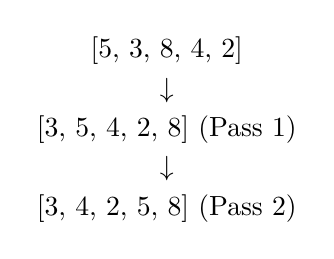
\begin{tikzpicture}
    \node at (0,2) {[5, 3, 8, 4, 2]};
    \node at (0,1.5) {$\downarrow$};
    \node at (0,1) {[3, 5, 4, 2, 8] (Pass 1)};
    \node at (0,0.5) {$\downarrow$};
    \node at (0,0) {[3, 4, 2, 5, 8] (Pass 2)};
\end{tikzpicture}
\captionof{figure}{Bubble Sort Passes}
\end{center}
\end{solutionbox}

\begin{mnemonicbox}
\mnemonic{CABS - Compare Adjacent, Bubble-up Swapping}
\end{mnemonicbox}

\questionmarks{4(c) OR}{7}{Explain the working of quick sort method with example.}

\begin{solutionbox}
Quick sort selects a pivot and partitions the array.

\begin{center}
\captionof{table}{Quick Sort Steps}
\begin{tabulary}{\linewidth}{|C|L|}
\hline
1 & Choose Pivot \\ \hline
2 & Partition: Small go Left, Large go Right \\ \hline
3 & Recursively sort Left and Right subarrays \\ \hline
\end{tabulary}
\end{center}

\begin{center}
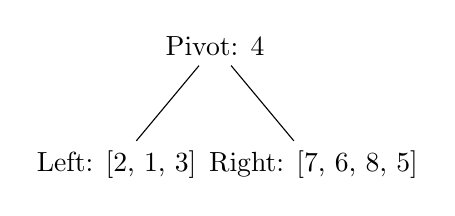
\begin{tikzpicture}[level distance=1.5cm, sibling distance=2.5cm]
    \node {Pivot: 4}
    child {node {Left: [2, 1, 3]}}
    child {node {Right: [7, 6, 8, 5]}};
\end{tikzpicture}
\captionof{figure}{Quick Sort Partition}
\end{center}
\end{solutionbox}

\begin{mnemonicbox}
\mnemonic{PPR - Pivot, Partition, Recursive divide}
\end{mnemonicbox}

\questionmarks{5(a)}{3}{Explain binary tree.}

\begin{solutionbox}
A binary tree is a hierarchical data structure where each node has at most two children.

\begin{center}
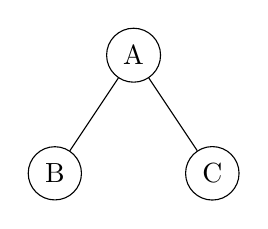
\begin{tikzpicture}[level distance=1.5cm, sibling distance=2cm]
    \node [circle, draw] {A}
    child {node [circle, draw] {B}}
    child {node [circle, draw] {C}};
\end{tikzpicture}
\captionof{figure}{Binary Tree}
\end{center}
\end{solutionbox}

\begin{mnemonicbox}
\mnemonic{RLTM - Root, Left, Two, Maximum}
\end{mnemonicbox}

\questionmarks{5(b)}{4}{Define the terms root, path, parent and children with reference to tree.}

\begin{solutionbox}
\begin{center}
\captionof{table}{Tree Terminology}
\begin{tabulary}{\linewidth}{|L|L|}
\hline
\textbf{Term} & \textbf{Definition} \\ \hline
\textbf{Root} & Topmost node with no parent \\ \hline
\textbf{Path} & Sequence of connected nodes \\ \hline
\textbf{Parent} & Node with one or more children \\ \hline
\textbf{Children} & Nodes connected to a parent \\ \hline
\end{tabulary}
\end{center}
\end{solutionbox}

\begin{mnemonicbox}
\mnemonic{RPPC - Root at Top, Path connects, Parent above, Children below}
\end{mnemonicbox}

\questionmarks{5(c)}{7}{Apply preorder and postorder traversal for given below tree.}

\begin{solutionbox}
Tree: 40(Root), Left:30, Right:50...

\begin{center}
\captionof{table}{Traversals}
\begin{tabulary}{\linewidth}{|L|L|L|}
\hline
\textbf{Traversal} & \textbf{Order} & \textbf{Result} \\ \hline
\textbf{Preorder} & Root, Left, Right & 40, 30, 25, 15, 28, 35, 50, 45, 60, 55, 70 \\ \hline
\textbf{Postorder} & Left, Right, Root & 15, 28, 25, 35, 30, 45, 55, 70, 60, 50, 40 \\ \hline
\end{tabulary}
\end{center}
\end{solutionbox}

\begin{mnemonicbox}
\mnemonic{PRE-NLR, POST-LRN}
\end{mnemonicbox}

\questionmarks{5(a) OR}{3}{Enlist applications of binary tree.}

\begin{solutionbox}
\begin{itemize}
    \item Binary Search Trees (Efficient searching)
    \item Expression Trees (Compilers)
    \item Huffman Coding (Compression)
    \item Priority Queues (Heaps)
    \item Decision Trees (ML)
\end{itemize}
\end{solutionbox}

\begin{mnemonicbox}
\mnemonic{BEHPD}
\end{mnemonicbox}

\questionmarks{5(b) OR}{4}{Explain insertion of a node in binary search tree.}

\begin{solutionbox}
BST Property: Left $<$ Node $<$ Right.

\begin{enumerate}
    \item Start at root.
    \item If New $<$ Current, go Left.
    \item If New $>$ Current, go Right.
    \item Insert at empty spot.
\end{enumerate}

\begin{center}
\begin{tikzpicture}[node distance=1.5cm]
    \node [gtu state] (start) {Start};
    \node [gtu decision, below=of start] (check) {Compare};
    \node [gtu state, left=of check] (left) {Go Left};
    \node [gtu state, right=of check] (right) {Go Right};
    \node [gtu state, below=of check] (insert) {Insert};
    
    \draw [gtu arrow] (start) -- (check);
    \draw [gtu arrow] (check) -- node[above] {Smaller} (left);
    \draw [gtu arrow] (check) -- node[above] {Larger} (right);
    \draw [gtu arrow] (left) |- (insert);
    \draw [gtu arrow] (right) |- (insert);
\end{tikzpicture}
\captionof{figure}{BST Insertion}
\end{center}
\end{solutionbox}

\begin{mnemonicbox}
\mnemonic{LSRG}
\end{mnemonicbox}

\questionmarks{5(c) OR}{7}{Draw Binary search tree for 8, 4, 12, 2, 6, 10, 14, 1, 3, 5 and write In-order traversal for the tree.}

\begin{solutionbox}
\begin{center}
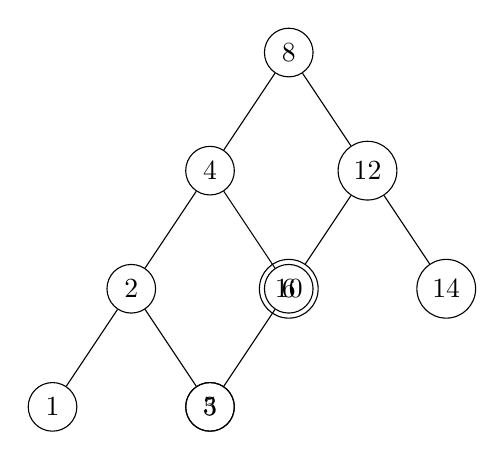
\begin{tikzpicture}[level distance=1.5cm, sibling distance=2cm]
    \node [circle, draw] {8}
    child {node [circle, draw] {4}
        child {node [circle, draw] {2}
            child {node [circle, draw] {1}}
            child {node [circle, draw] {3}}
        }
        child {node [circle, draw] {6}
            child {node [circle, draw] {5}}
            child[missing]
        }
    }
    child {node [circle, draw] {12}
        child {node [circle, draw] {10}}
        child {node [circle, draw] {14}}
    };
\end{tikzpicture}
\captionof{figure}{Constructed BST}
\end{center}

\textbf{In-order Traversal (Left, Root, Right):} \\
1, 2, 3, 4, 5, 6, 8, 10, 12, 14
\end{solutionbox}

\begin{mnemonicbox}
\mnemonic{LNR - Left, Node, Right}
\end{mnemonicbox}

\end{document}
